\section{Problem Formulation}
\label{sec:problem_formulation}
In this section, we first introduce the system and threat model, and then discuss the design goals of our system.

\subsection{System Model}
\label{subsec:system_model}

We consider the scenario where the users are having a conversation in an indoor environment such as an office or a meeting room. The users may need to record the conversation while they also want to prevent the conversation from being eavesdropped by possible unknown adversaries. As shown in Figure \ref{fig:system_model}, the system involves four entities:


\begin{figure}[t]
    \centering
    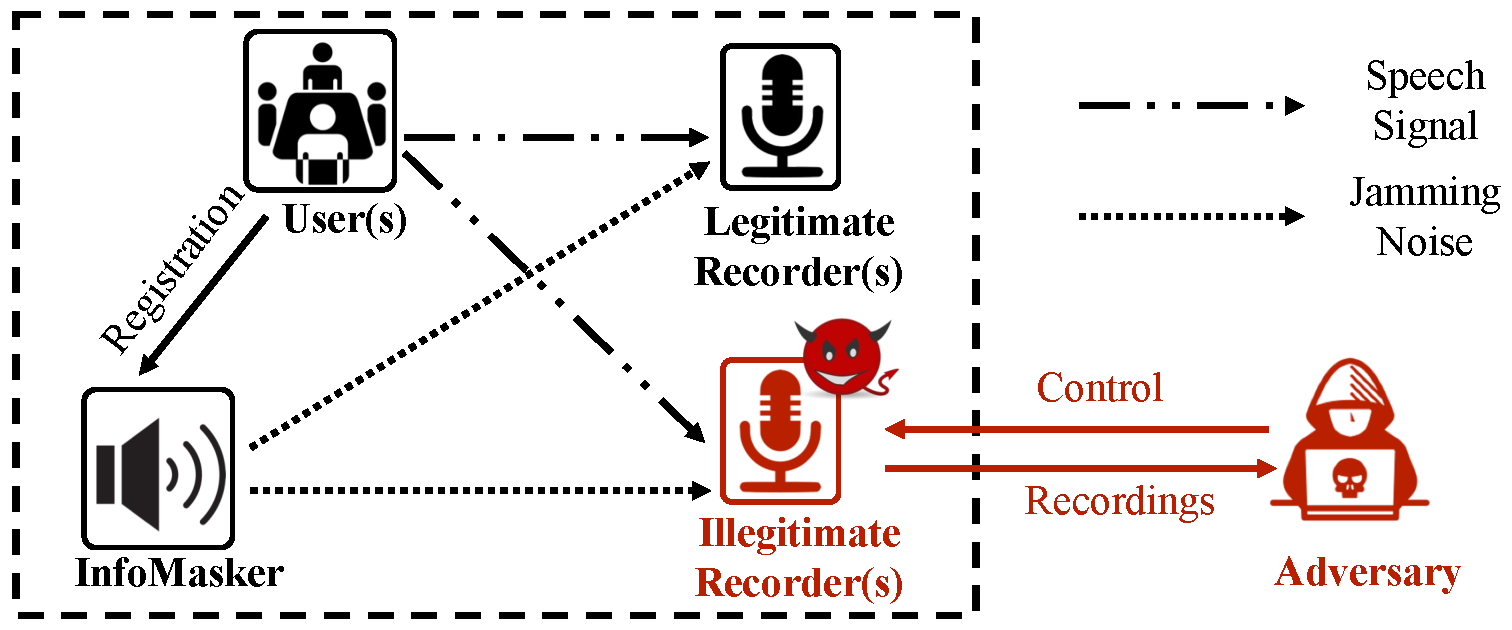
\includegraphics[width=\linewidth]{./images/system_model.pdf}
    \caption{System Model.}
    \label{fig:system_model}
    \vspace{-7mm}
\end{figure}

\textbf{User(s) }are the people who are having a conversation. To safeguard their privacy, they deploy \textit{InfoMasker} to prevent their voice from being eavesdropped.

\textbf{InfoMasker }is a user-controlled jamming device which can generate and emit jamming noise according to the users' registration information to prevent possible eavesdropping. Please note that we do not cover the voice call scenario since all microphones in the environment will be jammed.

% \textbf{InfoMasker }is a user-controlled jamming device designed to generate customized jamming noise according to the users' registration information. The noise is then broadcast towards nearby recorders to make the recordings unrecognizable to both humans and machines. Please note that we do not cover the voice call scenario since all microphones in the environment will be jammed.

\textbf{Legitimate Recorder(s) }are placed by the users to record the ongoing conversation. Because of the presence of InfoMasker, the recorded audios will also be affected and will contain both the conversation and the jamming noise. After the conversation, the users will try to recover the content from the noisy recording. Comparing to the adversary, the users know the detail of the injected noise.

\textbf{Illegitimate Recorder(s) }refer to all other devices equipped with microphones in the environment, such as smartphones and smart watches. Due to the black box nature of most electronic products, they are not fully controlled by users and may eavesdrop on users secretly. Considering the ease of use, users are unlikely to put these devices in hidden areas which may cause non-line-of-sight (NLOS), so here we do not consider the NLOS scenario.

\subsection{Threat Model}
We consider an adversary who can control recording devices in the environment (e.g., the manufacturer of the smart home devices). To eavesdrop on the content of the conversation, the adversary would record the speech signals, improve the recordings' intelligibility using various methods, and then extract semantic information. In this work, we assume the adversary has the following capabilities in each step of eavesdropping:

\textbf{Audio Recording. }We assume the adversary can control one or more recording devices in the environment to record single-channel or multi-channel audio signals.

\textbf{Speech Enhancement.}
We assume that the adversary can improve intelligibility of the recorded speech signals with different speech enhancement methods, including noise reduction, speech separation, and Blind Signal Separation (BSS) if multi-channel recordings are acquired.

\textbf{Semantic Information Extraction. }We consider that the adversary could jointly use different ASRs together with human ear to extract semantic information from the enhanced recordings, where human can recognize recordings accurately and ASRs can interpret speech contents efficiently. 

We also consider a powerful adversary who knows details of our noise generation method and could train a customized ASR system targeting on our noise.


\subsection{Design Goals}
We envision the following design goals of InfoMasker:

\textbf{Effectiveness}: 
Noise transmitted by InfoMasker should be able to prevent both ASR systems and the human auditory system from recognizing the noisy recording, which contains voices from single or multiple users.

\textbf{Robustness}: Noise injected by InfoMasker should be robust against various speech enhancement methods.

\textbf{Low-interference}: Noise signal transmitted by InfoMasker should be inaudible and harmless to human beings.

\textbf{Controlled Recording Privilege}: Users with the recording privilege can recover the content from noisy recordings.
